\documentclass[12pt]{article}
\usepackage[utf8]{inputenc}
\usepackage[T1]{fontenc} % uses T1 fonts (better quality)
\usepackage{lmodern}
\usepackage[dvipsnames]{xcolor}
\usepackage[margin=2cm]{geometry}
\geometry{top=1.5cm}
\usepackage{graphicx} \graphicspath{ {./Images/} }
\usepackage{pdfpages}
\usepackage{booktabs}   % for table borders
\usepackage{amsmath,bm,amssymb}
\usepackage{mathtools}
\usepackage[makeroom]{cancel}
\usepackage{tikz} \usetikzlibrary{shapes,arrows}
\usepackage{minted} \usemintedstyle{friendly}
\usepackage{enumitem}
\makeatletter
\renewcommand{\thefigure}{7.\@arabic\c@figure}
\makeatother
\begin{document}
 	\begin{center}
    \line(1,0){300}\\[0.25cm]
 	\Large{\bfseries ECE540: Homework \#3}\\
 	\textsc{\large David Kirby}\\
 	\textsc{\large Due: 12 October 2020}\\
 	\line(1,0){300}\\[0.75cm]
 	\end{center}
% Define block styles
% \tikzstyle{decision} = [diamond, draw, fill=blue!20,
%     text width=4.5em, text badly centered, node distance=3cm, inner sep=0pt]
% \tikzstyle{block} = [rectangle, draw,
%     text width=20em, text centered, rounded corners, minimum height=1em]
% \tikzstyle{line} = [draw, -latex']
% \tikzstyle{cloud} = [draw, ellipse,fill=red!20, node distance=3cm,
%     minimum height=2em]
% \noindent
\section*{Chapter 7 (\(\bm{7^{th}}\) Edition)}
\subsection*{Review Questions}
\begin{enumerate}
\item R4. As a mobile node gets farther and farther away from a base station, what are two actions that a base station could take to ensure that the loss probability of a transmitted frame does not
increase?
\begin{itemize}
	\item Increase the signal-to-noise ratio (SNR) by increasing the transmission power.
	\item Decrease the bit error rate (BER) by decreasing the transmission rate.
\end{itemize}
\item R7. Why are acknowledgments used in 802.11 but not in wired Ethernet?\\[1em]
Wireless channels are prone to higher levels bit rate errors. Acknowledgements are used in 802.11 to mitigate these errors. Wired Ethernet does not suffer the same level of bit rate errors.
\item R8. True or false: Ethernet and 802.11 use the same frame structure.\\[1em]
False
\item R14. What is the role of the “core network” in the 3G cellular data architecture?\\[1em]
The 3G core cellular data network connects radio access networks to the public Internet and interoperates with components of the existing cellular voice network.
\item R17. What are three important differences between 3G and 4G cellular ­architectures?
\begin{itemize}
	\item 4G has a unified, all-IP network architecture, unlike the 3G network, which has separate network components and paths for voice and data traffic.
	\item 4G has a clear separation of the data plane and the control plane.
	\item 4G has a clear separation between the radio access network and the all-IP-core ­network.
\end{itemize}
\item R19. What is the difference between a permanent address and a care-of address? Who assigns a care-of address?\\[1em]
Permanent address is the IP address on a mobile node's home network, while a care-of address is temporary and when a mobile node is on a foreign network. In the case of care-of addresses, the foreign network will assign the address.
\item R21. What are the purposes of the HLR and VLR in GSM networks? What elements of mobile IP are similar to the HLR and VLR?\\[1em]
The Home  Location  Register (HLR) contains the permanent cell phone number, location, and subscriber profile of each subscriber. The visitor location register (VLR) is temporary and contains entries for each of the visiting mobile users currently on its section of the network.
\item R23. What are three approaches that can be taken to avoid having a single ­wireless link degrade the performance of an end-to-end transport-layer TCP ­connection?
\begin{itemize}
	\item Local recovery.
	\item TCP sender awareness of wireless links.
	\item Split-connection approaches.
\end{itemize}
\end{enumerate}
\subsection*{Problems}
\begin{enumerate}
	\item P5. Suppose there are two ISPs providing WiFi access in a particular café, with each ISP operating its own AP and having its own IP address block.
	\begin{enumerate}
		\item Further suppose that by accident, each ISP has configured its AP to operate over channel 11. Will the 802.11 protocol completely break down in this situation? Discuss what happens when two stations, each associated with a different ISP, attempt to transmit at the same time.\\[1em]
		Even though the APs are broadcasting over the same channel (channel 11 indicates this is on the 2.4 GHz band), they will still have different SSIDs and MAC addresses. The protocol also has fail-safes such that it will \underline{not} completely break down. There will, however, be a higher likelihood of collision, but 802.11 has collision avoidance protocols in place.
		\item Now suppose that one AP operates over channel 1 and the other over channel 11. How do your answers change?\\[1em]
		In the case of two APs operating on non-overlapping channels, there would be no interference and therefore, in an ideal situation, no signal degradation.
	\end{enumerate}
	\item P7. Suppose an 802.11b station is configured to always reserve the channel with the RTS/CTS sequence. Suppose this station suddenly wants to ­transmit 1,000 bytes of data, and all other stations are idle at this time. As a ­function of SIFS and DIFS, and ignoring propagation delay and assuming no bit errors, calculate the time required to transmit the frame and receive the acknowledgment.
	\begin{align*}
		\text{t}_{\text{RTS/CTS}}&=\frac{32\text{ bytes}}{11\text{ Mbps}}\\
		&=23.27\ \mu \text{s}\\
		\text{t}_{\text{data}}&=\frac{1000\text{ bytes}+32\text{ bytes}}{11\text{ Mbps}}\\
		&=750.55\ \mu \text{s}
	\end{align*}
	\begin{align*}
		\text{t}_{\text{total}}&=\text{DIFS + RTS + SIFS + CTS + SIFS + Data + SIFS + ACK}\\
		&=\text{DIFS + }23.27\ \mu \text{s}+\text{SIFS}+23.27\ \mu \text{s}+\text{SIFS}+750.55\ \mu \text{s}+\text{SIFS}+23.27\ \mu \text{s}\\
		&=820.36\ \mu \text{s}+ \text{DIFS + }3\cdot \text{SIFS}
	\end{align*}
	\item P8. Consider the scenario shown in Figure 7.34, in which there are four wireless nodes, A, B, C, and D. The radio coverage of the four nodes is shown via the shaded ovals; all nodes share the same frequency. When A transmits, it can only be heard/received by B; when B transmits, both A and C can hear/receive from B; when C transmits, both B and D can hear/receive from C; when D transmits, only C can hear/receive from D.
	\setcounter{figure}{33}
		\begin{figure}[h!]
		\centering
		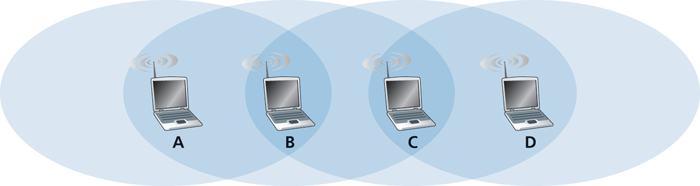
\includegraphics[width=0.85\textwidth]{./Images/Fig07-031.png}
		\caption{Scenario for problem P8}
		% \label{fig:I2Cdemo}
		\end{figure}\\
		Suppose now that each node has an infinite supply of messages that it wants to send to each of the other nodes. If a message’s destination is not an immediate neighbor, then the message must be relayed. For example, if A wants to send to D, a message from A must first be sent to B, which then sends the message to C, which then sends the message to D. Time is slotted, with a message transmission time taking exactly one time slot, e.g., as in slotted Aloha. During a slot, a node can do one of the following: (i) send a message, (ii) receive a message (if exactly one message is being sent to it), (iii) remain silent. As always, if a node hears two or more simultaneous transmissions, a collision occurs and none of the transmitted messages are received successfully. You can assume here that there are no bit-level errors, and thus if exactly one message is sent, it will be received correctly by those within the transmission radius of the sender.
	\begin{enumerate}
		\item Suppose now that an omniscient controller (i.e., a controller that knows the state of every node in the network) can command each node to do whatever it (the omniscient controller) wishes, i.e., to send a message, to receive a message, or to remain silent. Given this omniscient controller, what is the maximum rate at which a data message can be transferred from C to A, given that there are no other messages between any other source/destination pairs?
		\begin{align*}
			1 \text{ message}/2 \text{ time slots \bigg\{ }C \rightarrow B \rightarrow A
		\end{align*}
		\item Suppose now that A sends messages to B, and D sends messages to C. What is the combined maximum rate at which data messages can flow from A to B and from D to C?
		\[
			\text{2 messages/1 time slot}
			\begin{dcases*}
			A \rightarrow B\\
		    D \rightarrow C
			\end{dcases*}
		\]
		\item Suppose now that A sends messages to B, and C sends messages to D. What is the combined maximum rate at which data messages can flow from A to B and from C to D?\\[1em]
		This time, there will be a collision because B is hearing both A and C. B will fail to receive from A and have to wait. D however only hears C, so it will receive in the first time slot.
		\begin{align*}
			1 \text{ message}/1 \text{ time slot \bigg\{ }C \rightarrow D; &\quad A \rightarrow B
		\end{align*}
		\item Suppose now that the wireless links are replaced by wired links. Repeat questions (a) through (c) again in this wired scenario.\\[1em]
		(a) and (b) would remain the same as for wireless since in scenario (a) C is sill not directly connected to A, and in scenario (b) the wired link would still send two messages per time slot. In (c), however, we would be able to send two messages per time slot due to direct links between the nodes (and lack of collision).
		\item Now suppose we are again in the wireless scenario, and that for every data message sent from source to destination, the destination will send an ACK message back to the source (e.g., as in TCP). Also suppose that each ACK message takes up one slot. Repeat questions (a)--(c) above for this scenario.\\[1em]
		This would effectively double the time slots needed for the RTT of each of the data messages. For (a) we would be looking a 1 message/4 time slots, (b) 2 messages/2 time slots, and (c) 1 message/2 time slots.
	\end{enumerate}
	\item P11. In Section 7.5, one proposed solution that allowed mobile users to maintain their IP addresses as they moved among foreign networks was to have a foreign network advertise a highly specific route to the mobile user and use the existing routing infrastructure to propagate this information throughout the network. We identified scalability as one concern. Suppose that when a mobile user moves from one network to another, the new foreign network advertises a specific route to the mobile user, and the old foreign network withdraws its route. Consider how routing information propagates in a distance-vector algorithm (particularly for the case of interdomain routing among networks that span the globe).
	\begin{enumerate}
		\item Will other routers be able to route datagrams immediately to the new foreign network as soon as the foreign network begins advertising its route?\\[1em]
		The other routers will \underline{not} be able to route datagrams immediately as it would take time for the advertised routes to propagate throughout the system.
		\item Is it possible for different routers to believe that different foreign networks contain the mobile user?\\[1em]
		It is possible as it takes time for the information to propagate between the foreign networks.
		\item Discuss the timescale over which other routers in the network will eventually learn the path to the mobile users.\\[1em]
		The time it takes for the updated information to propagate depends on the number of hops between the edge router and the updated router.
	\end{enumerate}
	\item P15. Consider two mobile nodes in a foreign network having a foreign agent. Is it possible for the two mobile nodes to use the same care-of address in mobile IP? Explain your answer.\\[1em]
	It is entirely possible for two mobile nodes to use the same care-of address (COA). If two mobile nodes visit the same foreign network and have the same foreign agent, they could be assigned the same COA.
\end{enumerate}
\end{document}